\chapter{Technologien}

\section{Oculus Quest 3}

\section{WebGL}

\section{WebXR}

WebXR ist eine standartisierte API für Webanwendungen, welche es ermöglicht, immersive VR und AR Anwendungen für das Internet zu erstellen.
Das World Wide Web Consortium (W3C), welches die WebXR-Standarts definiert beschreibt WebXR wie folgt: \glqq{}Die WebXR Device API bietet die notwendigen Schnittstellen, damit Entwickler ansprechende, komfortable und sichere immersive Anwendungen im Web für eine Vielzahl von Hardware-Formfaktoren erstellen können.\grqq{} \autocite[aus dem Englischen mit DeepL ][1. Introduction]{w3c_webxr}
Mit WebXR entwickelte Anwendungen können als Webanwendungen direkt von einem Webbrowser eines AR- oder VR-Geräts aus aufgerufen werden, ohne dass eine zusätzliche Installation der Anwendung notwendig ist.

\begin{figure}[H]
    \centering
    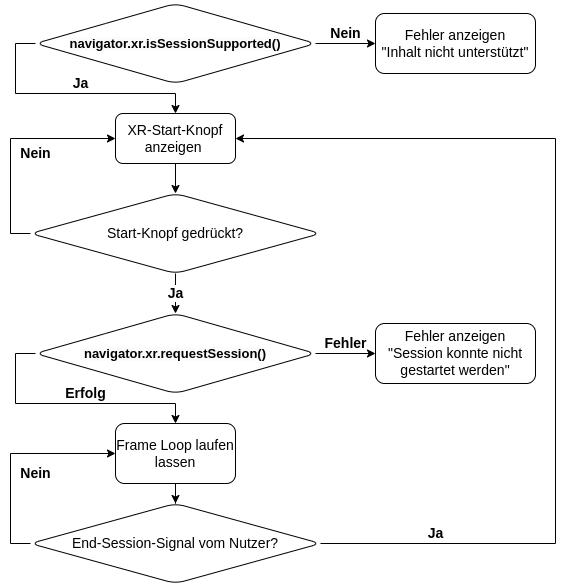
\includegraphics[width=0.5\textwidth]{images/WebXR-App-Flow.png}
    \caption{Application Flow von WebXR-Anwendungen}
    \source{ Eigene Darstellung nach \autocite[][1.2. Application Flow]{w3c_webxr}}
    \label{fig:webxr-app-flow}
  \end{figure}

Der Flow von WebXR-Anwendungen ist in Abbildung \ref{fig:webxr-app-flow} dargestellt.
Dabei wird zuerst beim Aufrufen der Anwendung geprüft, ob die angegebene Art von XR-Inhalt von der Hardware und dem User Agent (UA), also der Software mit der der Nutzer auf den Inhalt zugreift, unterstützt werden.
Ist dies der Fall, kann die XR-Session vom Nutzer manuell gestartet werden.
Startet die Session erfolgreich wird der Frame Loop der Anwendung gestartet.
Der Frame Loop ist eine Schleifenfunktion, die kontinuierlich während der XR-Session ausgeführt wird um die einzelnen Frames, bzw. Bilder, für das XR-Display zu rendern.
Dieser Frame Loop läuft, bis die Session durch den UA beendet wird.
Befindet sich der UA noch auf der Seite der WebXR-Anwendung, wird wieder der Knopf zum Starten der XR-Session angezeigt, falls der Nutzer direkt wieder eine neue Session starten möchte.

\subsection{Three.js}

\subsection{A-Frame}

\subsection{PlayCanvas}

\subsection{Babylon.js}

\section{Android Debug Bridge}